\documentclass[tikz]{standalone}
\usetikzlibrary{intersections}
\begin{document}
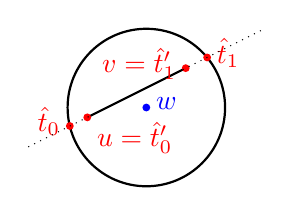
\begin{tikzpicture}
  \coordinate (u0) at (-1.5,-0.5);
  \coordinate (u) at (-0.75,-0.125);
  \coordinate (v) at (0.5,0.5);
  \coordinate (v0) at (1.5,1);
  \coordinate (w) at (0,0);

  \draw[thick] (u) -- (v);
  \draw[thick] (w) circle (1);

  % Find intersection points between the line and the circle
  \path[name path=line] (u0) -- (v0);
  \path[name path=circle] (w) circle (1);
  \path[name intersections={of=line and circle, by={t1,t0}}];

  \node[circle,fill,color=red,inner sep=1pt,label={[text=red, below right]:\(u=\hat t_0'\)}] at (u) [] {}; 
  \node[circle,fill,color=red,inner sep=1pt,label={[text=red, left]:\(v=\hat t_1'\)}] at (v) [] {}; 
  \node[circle,fill,color=blue,inner sep=1pt,label={[text=blue,right]:\(w\)}] at (w) [] {}; 

  \node[circle,fill,color=red,inner sep=1pt,label={[text=red, left]:\(\hat t_0\)}] at (t0) [] {}; 
  \node[circle,fill,color=red,inner sep=1pt,label={[text=red, right]:\(\hat t_1\)}] at (t1) [] {}; 

  \draw[dotted] (u0) -- (v0);
\end{tikzpicture}
\end{document}
